\section{Nguồn dữ liệu và kiến trúc hệ thống}
\subsection{Dữ liệu nguồn}
Nguồn là Brazilian E-Commerce Public Dataset by Olist (Kaggle) \cite{olist}, gồm chín tệp CSV đi kèm dự án. Số bản ghi được đếm bằng bộ phân tích CSV chuẩn (không đếm dòng văn bản vì trường nhận xét có thể chứa xuống dòng).

\begin{table}[H]\centering\small
\begin{tabularx}{\linewidth}{Yrr}
\toprule Tệp CSV (rút gọn tên) & Số bản ghi & Được nạp\\\midrule
customers & 99.441 & Có \\
orders & 99.441 & Có \\
order\_items & 112.650 & Có \\
order\_payments & 103.886 & Có \\
products & 32.951 & Có \\
sellers & 3.095 & Có \\
product\_category\_name\_translation & 71 & Có \\
geolocation & 1.000.163 & Không \\
order\_reviews & 99.224 & Không \\
\bottomrule\end{tabularx}
\caption{Kiểm kê dữ liệu nguồn}
\end{table}

Bảy tệp được nạp (khai báo trong \code{RAW_TABLE_FILES}). Khách hàng có hai mã, trong đó \code{customer_id} nối với đơn, còn \code{customer_unique_id} nhận diện một người mua qua nhiều đơn. Bảng sản phẩm có thể thiếu danh mục; bản dịch được nối trái để không loại sản phẩm. Mỗi dòng order item là một mục trong đơn; \code{order_item_id} là số thứ tự trong đơn, không phải số lượng.

\subsection{Kiến trúc và luồng xử lý}
\begin{figure}[H]\centering
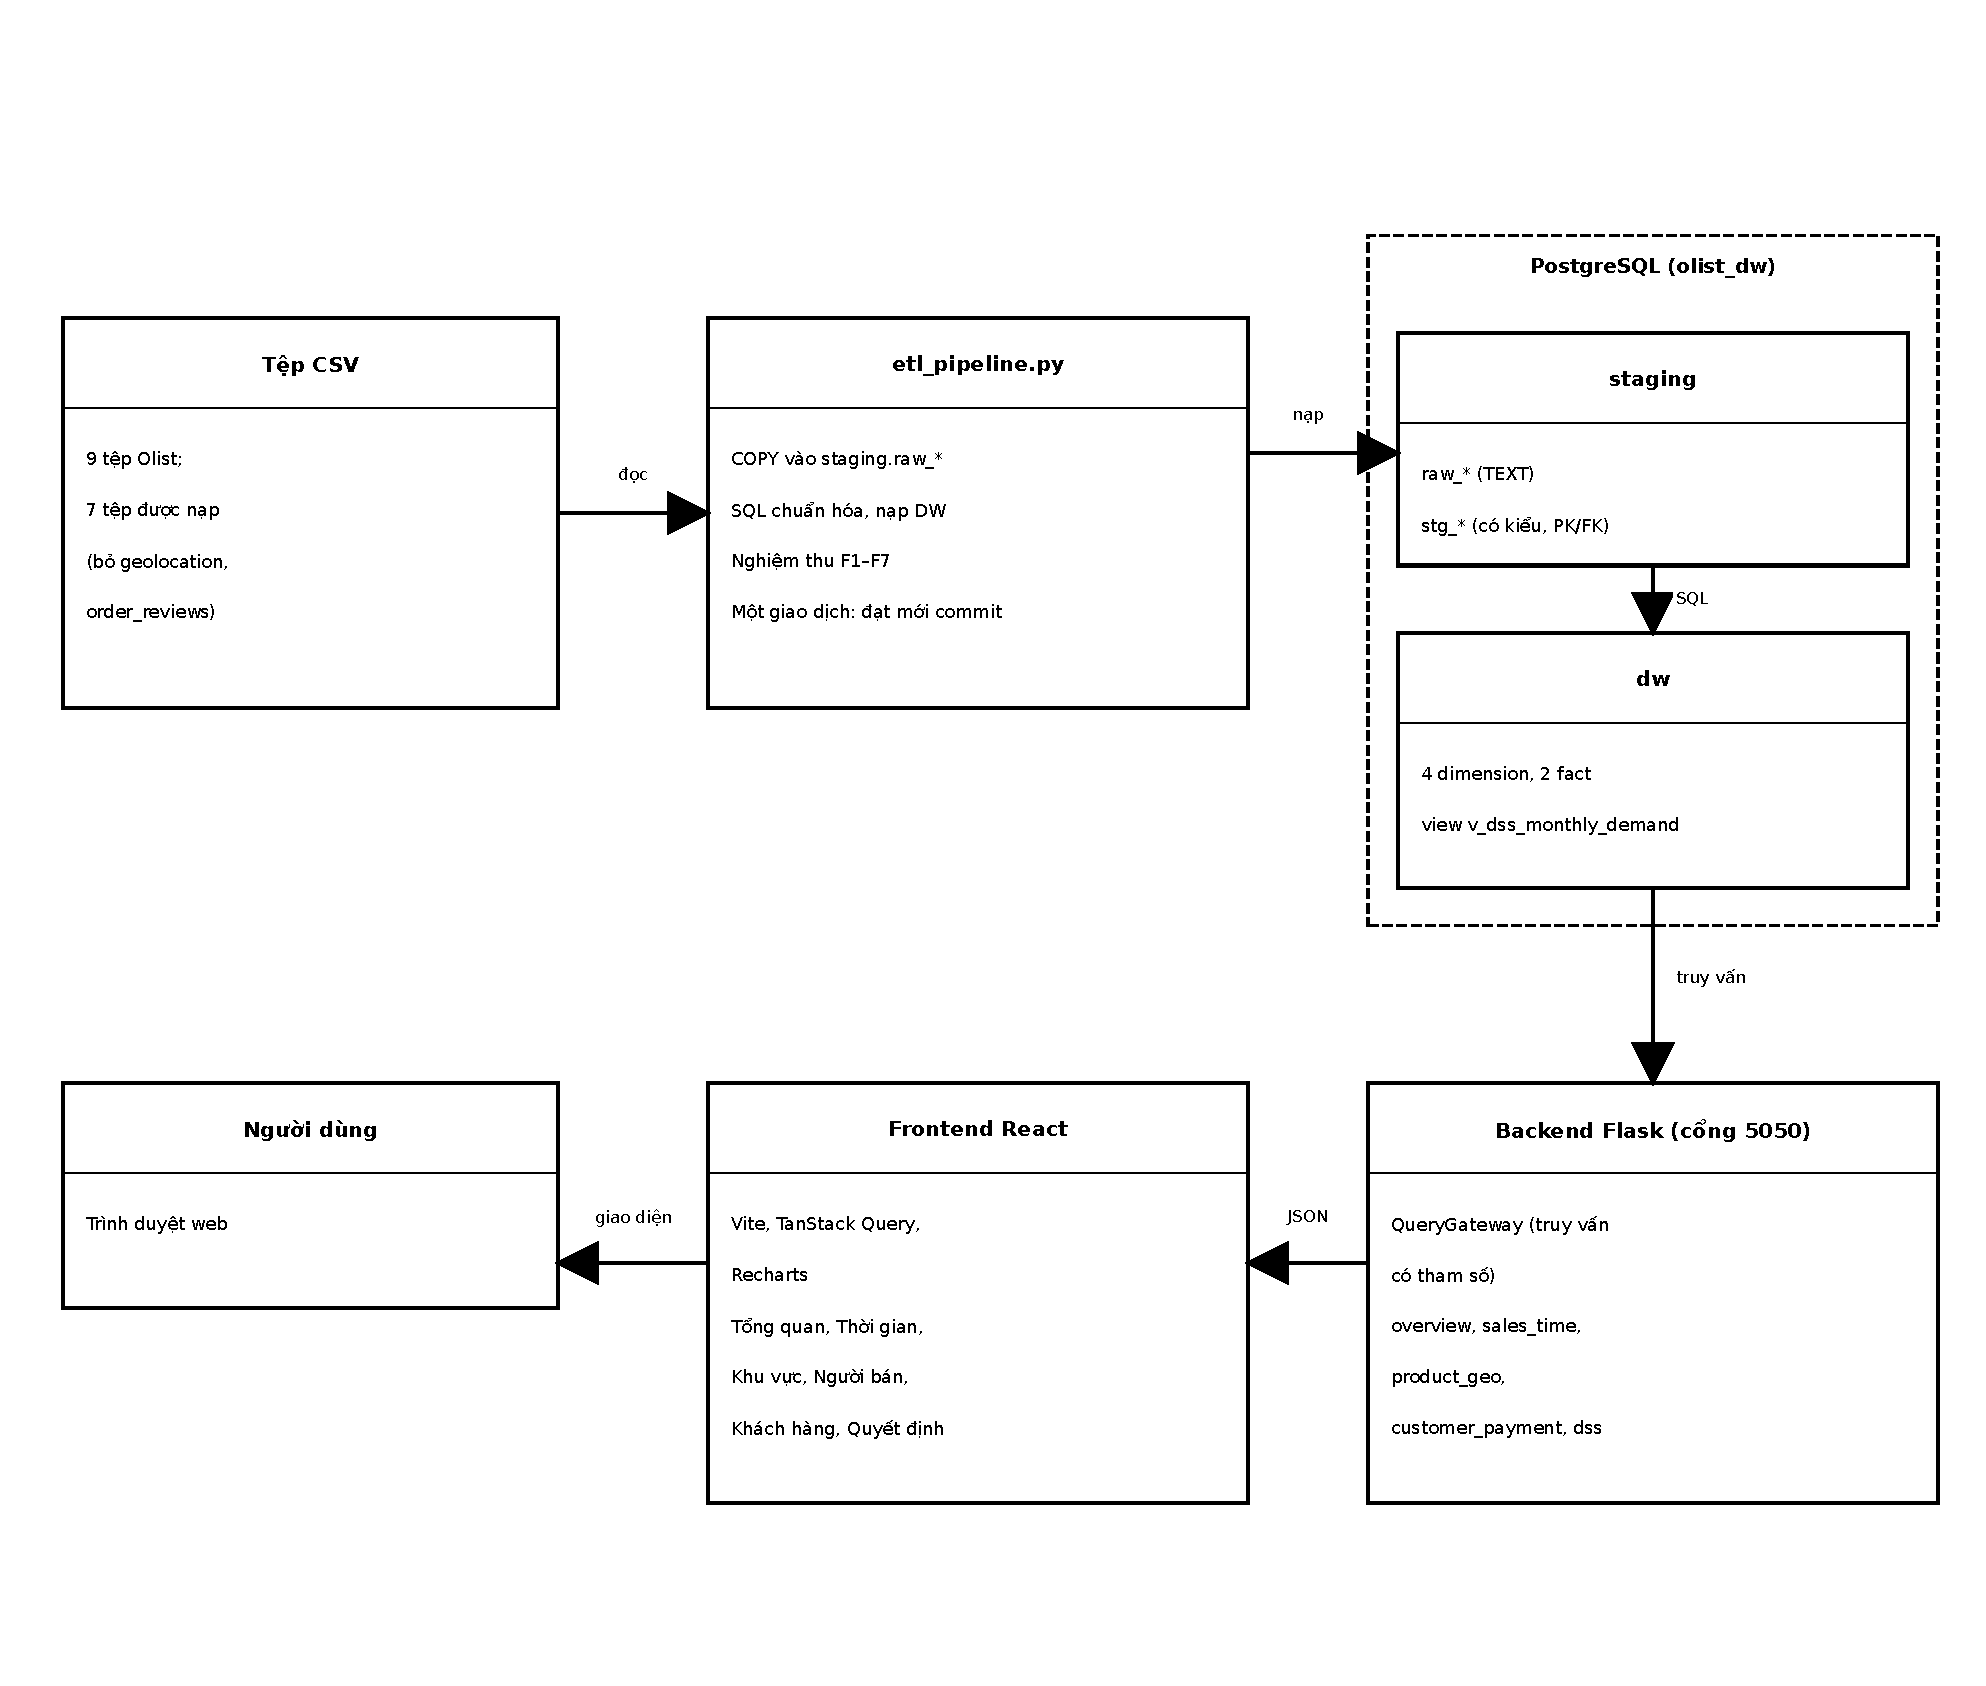
\includegraphics[width=\linewidth]{assets/fig_architecture.pdf}
\caption{Kiến trúc hệ thống}
\label{fig:architecture}
\end{figure}

Luồng xử lý gồm: (1) COPY các CSV vào \code{staging.raw_*} (toàn kiểu TEXT); (2) SQL chuẩn hóa sang \code{staging.stg_*} có kiểu và khóa; (3) SQL nạp \code{dw.dim_*} và hai bảng fact; (4) chạy bộ nghiệm thu; (5) tạo view nguồn cho DSS. Phép biến đổi chủ yếu diễn ra bằng SQL sau khi raw đã nằm trong PostgreSQL nên trình tự mang tính ELT; Python chỉ điều phối và nạp tệp bằng \code{copy_expert}. Backend Flask đọc kho qua một lớp truy vấn dùng chung; frontend React gọi API và vẽ biểu đồ.

\subsection{Công nghệ và cấu hình}
Backend dùng Flask, flask-cors và psycopg2; NumPy được dùng trong mô-đun dự báo DSS (cài kèm Pandas). SQLAlchemy và Pandas có trong \code{requirements.txt} vì \code{db_connect.py} dùng chung với các script chạy SQL, backend chỉ dùng hàm kết nối psycopg2 của tệp này. Lớp \code{QueryGateway} mở kết nối, thực thi truy vấn có tham số, chuyển kiểu kết quả sang JSON rồi đóng kết nối. API chạy ở cổng 5050. Frontend dùng React, TypeScript, Vite, TanStack Query, Recharts và Tailwind.

Kết nối cơ sở dữ liệu đọc từ tệp \code{.env} đặt cạnh \code{db_connect.py} (các biến \code{DB_HOST}, \code{DB_PORT}, \code{DB_NAME}, \code{DB_USER} và \code{DB_PASSWORD}). Chạy \code{python etl_pipeline.py} để nạp kho, rồi \code{python backend/run.py} và \code{npm run dev} trong \code{frontend}.
